

The PAK/PPK protocols were first introduced by Boyko, MacKenzie and Patel in \cite{BoMaPa00} in 2000
as a Diffie-Hellman based provably secure PAKEs. The PAK protocol contained explicit key confirmation
while PPK did not. An augmented version of it, namely PAK-Z, was also introduced in the same paper.

The setting of PAK/PPK is similar to all other Diffie-Hellman based PAKEs. What is different is its dependencies on perfect hash functions.

Let $\pi$ be the password. Let $p, q$ be large primes and $p = rq+1$, where $r, q$ are relatively prime. Let $g$ be a generator
of a subgroup of $\mathbb{Z}^\ast_p$ of size $q$ where the Decision Diffie-Hellman(DDH) problem
is infeasible. Let $H_1, H_{2a}, H_{2b}, H_3$ be independent random hash functions. The PAK and PPK
protocols are described as in Figures \ref{fig:pak} and \ref{fig:ppk}.

\begin{figure}[h]
    \label{fig:pak}
    \centering
    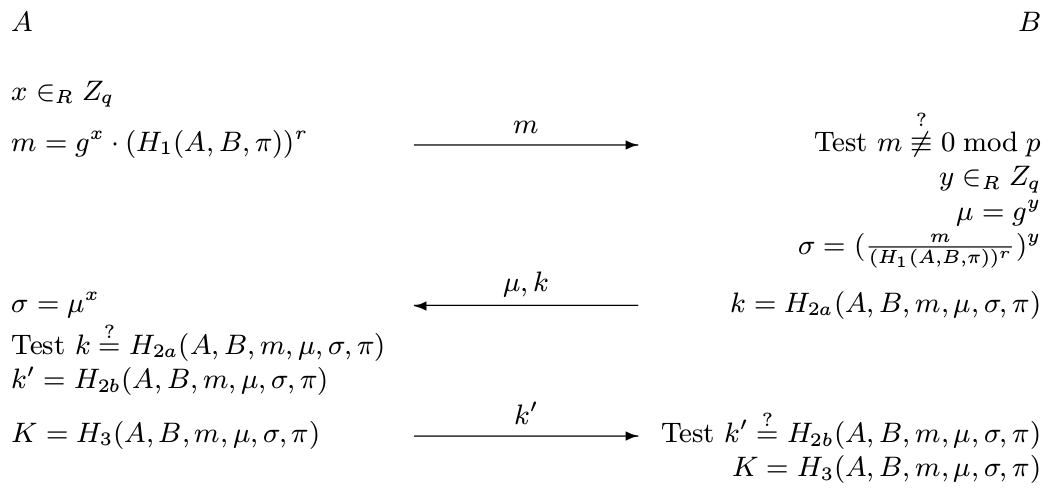
\includegraphics[scale=0.4]{pak_protocol.png}
    \caption{The PAK protocol.}
\end{figure}

\begin{figure}[h]
    \label{fig:ppk}
    \centering
    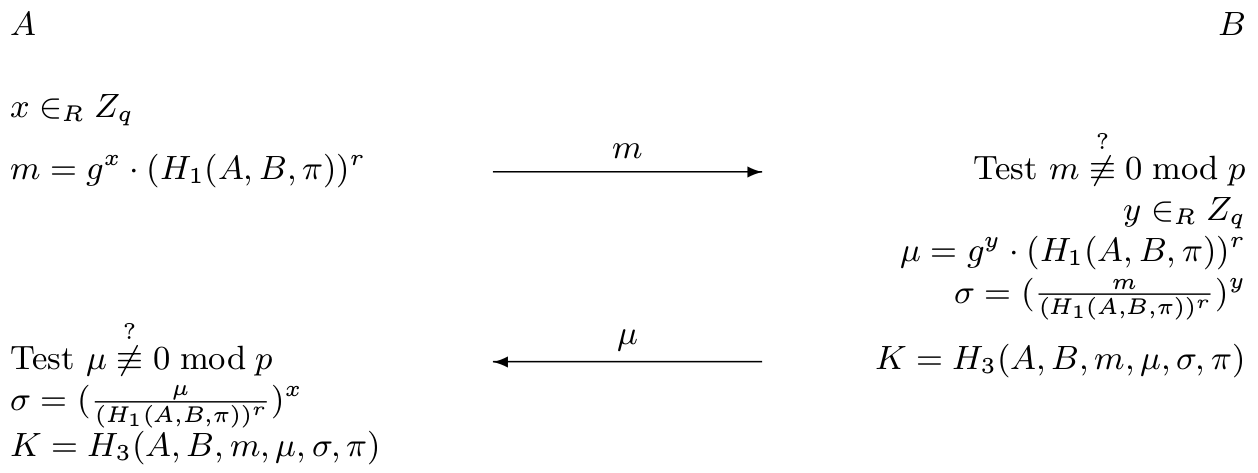
\includegraphics[scale=0.35]{ppk_protocol.png}
    \caption{The PPK protocol.}
\end{figure}


\iffalse
\begin{figure}[h]
    \begin{tikzpicture}
        \matrix (m)[matrix of nodes, column sep=2cm, row sep=8mm, nodes={draw=none, anchor=center, text depth=0pt}]{
            Alice                                          &                   & Bob                                       \\%line 1
            randomly choose $x \in \mathbb{Z}_q$ & & \\%line2
            $m= g^z\cdot(H_1(ID_{Alice}, ID_{Bob}, \pi))^r$ & $m$ &   Test $m\not\equiv 0\mod p$   \\%line3
            & & choose $y \in \mathbb{Z}_q$, $\mu = g^y$, $\sigma = \left(\frac{m}{H_1(ID_{Alice}, ID_{Bob}, \pi)}\right)^y$\\%line4
            Test $k = H_{2a}(ID_{Alice}, ID_{})$
        };

        % draw the nodes - these are 1-based indicies on the matrix called `m`, ie to draw in (x,y), reference it as `m-x-y`
        \draw[shorten <=-1.5cm,shorten >=-1.5cm] (m-1-1.south east)--(m-1-1.south west);    % underline "Alice"
        \draw[shorten <=-1.5cm,shorten >=-1.5cm] (m-1-3.south east)--(m-1-3.south west);    % underline "Bob"
        \draw[shorten <=-1cm,shorten >=-1cm,-latex] (m-3-2.south west)--(m-3-2.south east); % arrow below sending alpha^x_a
        \draw[shorten <=-1cm,shorten >=-1cm,-latex] (m-5-2.south east)--(m-5-2.south west); % arrow below sending alpha^x_b
    \end{tikzpicture}
    % if you do not need a caption, there's no need for the `figure` enviroment, a `tikzpicture` will be placed where ever you put
    % it in the code, unlike `figure` without [h] -- but you'll probably want a caption so these two lines are probably useless
    \label{fig:pak}
    \caption{The PAK protocol.}
\end{figure}

\fi















